In this section, we discuss a running example extracted from the c base-class library with
challenges of computing the symbolic
\emph{reachability-bound} on
every control location and illustrate how our algorithm leverages the challenges through the \emph{path reachability-bound} and the \emph{loop reachability-bound}.
% This example
% % is adopted from the example in~\cite{GulwaniZ10}, which
% is a skeleton code extracted from the c base-class library.

% \paragraph{Challenges.}
%\begin{example}
 % [The Running Example with Nested Loop in One Path]
%  \label{ex:relatedNestedWhileOdd-overview}
{ \small
% \vspace{-0.2cm}
\begin{figure}
\centering
\begin{subfigure}{.4\textwidth}
\begin{centering}
{\small
$
\begin{array}{l}
  \kw{nestedOdd}(n, m) \triangleq \\
  \clabel{ \assign{i}{n} }^{0} ; \\
      L_1: \ewhile ~ \clabel{i > 0}^{1} ~ \edo ~ \\
      \quad \big(
        \eif(\clabel{i \% 2 \neq 0 }^{2},
        \clabel{\assign{k}{i - m}}^{3};\\
        \quad L_4: \ewhile ~ \clabel{k > 0}^{4} \edo \\
        \quad ( \clabel{\assign{k}{k - 1}}^{5} );\\
        \quad \clabel{\assign{i}{k + m}}^{6};
        \clabel{\assign{i}{i - 1}}^{7}, \\
        \quad \clabel{\assign{i}{i - 3}}^{8})
        \big)
  \end{array}
$
}
\vspace{-0.3cm}
\caption{}
\end{centering}
\end{subfigure}
\begin{subfigure}{.52\textwidth}
\begin{centering}
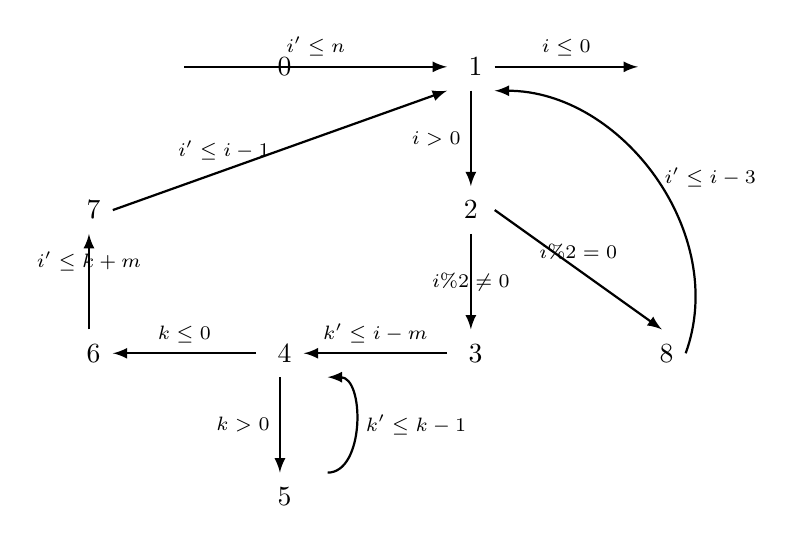
\begin{tikzpicture}[scale=\textwidth/20cm,samples=200]
\draw[] (-4, 10) circle (0pt) node{{ $0$}};
\draw[] (0, 10) circle (0pt) node{{ $1$}};
\draw[] (0, 7) circle (0pt) node{\textbf{$2$}};
\draw[] (0, 4) circle (0pt) node{{ $3$}};
\draw[] (-4, 4) circle (0pt) node{{ $4$}};
\draw[] (-8, 4) circle (0pt) node{{ $6$}};
\draw[] (-4, 1) circle (0pt) node{{ $5$}};
\draw[] (4, 4) circle (0pt) node{{ $8$}};
\draw[] (-8, 7) circle (0pt) node{{ $7$}};
% Counter Variables
\draw[] (4.5, 10) circle (0pt) node {\textbf{$\lex$}};
% \draw[] (6, 4) circle (0pt) node {{ $ex$}};
%
% Control Flow Edges:
\draw[ thick, -latex] (-6, 10)    -- node [above]{\scriptsize $i' \leq n$}(-0.5, 10);
\draw[ thick, -latex] (0, 9.5)    -- node [left] {\scriptsize $i > 0$} (0, 7.5) ;
\draw[ thick, -latex] (0.5, 7)    -- node [above] {\scriptsize $ i \% 2 = 0 $}  (4, 4.5);
\draw[ thick, -latex] (4.5, 4)    to  [out=70,in=0]   node [right] {\scriptsize $i' \leq i - 3$ }(0.5, 9.5);
\draw[ thick, -latex]  (0, 6.5)   -- node  {\scriptsize $i \% 2 \neq 0$}  (0, 4.5) ;
\draw[ thick, -latex]  (-0.5, 4)  -- node [above] {\scriptsize $k' \leq i - m$ }  (-3.5, 4) ;
\draw[ thick, -latex]  (-4.5, 4)  -- node [above] {\scriptsize $k \leq 0$ }  (-7.5, 4);
\draw[ thick, -latex] (0.5, 10)   -- node [above] {\scriptsize $i \leq 0$}  (3.5, 10);
\draw[ thick, -latex] (-4, 3.5)   -- node [left] {\scriptsize $k > 0$}  (-4, 1.5);
\draw[ thick, -latex] (-3, 1.5)   to  [out=0,in=0] node [right] {\scriptsize $k' \leq k- 1$}  (-3, 3.5);
\draw[ thick, -latex] (-8, 4.5)   --  node [above] {\scriptsize $i' \leq k + m$ }(-8, 6.5);
\draw[ thick, -latex] (-7.5, 7)  --  node [left] {\scriptsize $i' \leq i - 1$ }(-0.5, 9.5);
% \draw[ thick, -latex] (6, 6.5)  -- node [right] {$\top$} (6, 4.5) ;
\end{tikzpicture}
\vspace{-0.5cm}
\caption{}
\end{centering}
\end{subfigure}
\begin{subfigure}{.9\textwidth}    
\begin{centering}
{\small
$\tpath_0 = (0 \to 1)$
\quad
$\tpath_1 = (1 \to 2 \to 3 \to 4)$
\quad
$\tpath_2 = (4 \to 6 \to 7 \to 1)$
\quad
$\tpath_3 = (4 \to 5 \to 4)$
\quad
$\tpath_4 = (1 \to 2 \to 8 \to 1)$
\quad
$\tpath_5 = (1 \to \lex)$
}
\vspace{-0.3cm}
\caption{}
\end{centering}
\end{subfigure}
% \vspace{-0.5cm}
\begin{subfigure}{.8\textwidth}    
  \begin{centering}
  $
  \tpath_0 ; \rpchoose{ 1: \rprepeat(\tpath_1; 4:\rprepeat(\tpath_3); \tpath_2; \tpath_4), 
  1: \rprepeat(\tpath_4; \tpath_1; 4:\rprepeat(\tpath_3); \tpath_2) }; \tpath_5
  $
  % \vspace{-0.5cm}
  \caption{}
  \end{centering}
  \end{subfigure}
\caption{
(a) Running example: program with a loop with two  paths and a nested loop in one of them,
(b) the corresponding \emph{abstract transition graph}, $\absG(\kw{nestedOdd}(n, m))$,
(c) all the simple transition paths on this program,
(d) the refined program.}
% \vspace{-0.75cm}      
\label{fig:relatedNestedWhileOdd-overview}
\end{figure}
}
%  \footnotetext{In the transition path, $(l_0 \to \cdots \to l_n)$, the constraints are omitted for concise.}
%
%  \end{example}    

% \todo{Shorten}
% \begin{itemize}
% \item 
\textbf{Challenge I}
The example program in Figure~\ref{ex:relatedNestedWhileOdd-overview}(a) has two level nested loops, outer loop $L_1$ and nested loop $L_4$ which is in the first path of $L_1$. Given $n \geq m \geq 0$,
the expected \emph{reachability-bound}s for locations in outer loop $3, 6, 7$ and $8$ are all $\lfloor\frac{m}{4}\rfloor$,
% for $8$ is $\lfloor\frac{m}{4}\rfloor + 1$,
for location $2$ is $\lfloor\frac{m}{2}\rfloor$ and $\lfloor\frac{m}{2}\rfloor + 1$ for location $1$.
\highlight{Though within the same loop $L_1$, the bounds for different locations are different.}
The amortized analysis methodology such as Loopus~\cite{SinnZV17}, KoAT~\cite{BrockschmidtEFFG14,FalkeKS12,FalkeKS11}, C4B~\cite{CarbonneauxHS15}, etc. ignores path sensitivity and approximate the bound $n$ as the bound for loop $L_1$. 
While some path-refinement-based methods such as \cite{GulwaniZ10,GulwaniJK09}, CoFloCo~\cite{Montoya17,Flores-Montoya16,Flores-MontoyaH14} and etc. only give the same bound for all the locations within the loop $L_1$. 
Though we can reuse their results i.e., loop bounds as the \emph{reachability-bound} for location $1$ and $2$,
but it is still unclear for locations $3, 6, 7$, and $8$.
%
This motivates our first key novelty -- the \emph{path reachability-bound} $\inoutB(\rprog, \tpath)$ for a loop-free and interleaving-free path $\tpath$.
It bounds the evaluation times of each path over a path-refined program.
% \item 

\textbf{Challenge II} The second challenge occurs in the nested loop.
In line 6, since $i$ is reset by $k + m$ and $k$ is reset by $i - m$ at line 3, the
loop $L_4$ is only executed in the first iteration of while loop $L_1$.
% \\
The total iterations of the two loops are
$n - m + \lfloor\frac{m}{2}\rfloor + 1$,
and the tight \emph{reachability-bound} for location $5$ inside the $L_4$ is $m$.
% for locations $4, 5$ and $8$ between the $L_3$ and $L_6$ are $(n-N) \times (m - N)$,
% and $n - N$ for locations $2$ and $9$.
% \\
\highlight{The tight \emph{reachability-bound}s for the locations inside the loop $L_4$ is 
the same as its innermost loop iteration bound.
% , as well as our \emph{path reachability-bound}.
However, for the locations between $L_1$ and $L_4$,
the tight bounds are the multiplication of the inner and outer loop iteration bounds.}
% \\
% compute a better but still loose bound, $n + m^2 - m \times N$ on total iteration times.
The existing approach either ignores the path sensitivity or computes the same bound for all the locations in a loop.
None of them can give the precise \emph{reachability-bound}s for different locations in the loop,
which is non-trivial to compute even though knowing the loop bound.
% especially for the locations similar to $7$ in $\kw{threeNestedWhile}$.
This motivates us to consider our second novel quantity --
the numbers of iterations of the outer loop $L_1$ such that,
during these iterations, the loop $L_4$ is ``entered''. 

We refer to this quantity as the \emph{loop reachability} of the loop $L_4$ w.r.t the outer loop $L_1$.
% of the location within loop $L_6$ w.r.t the loops $L_3$ and $L_1$.
By multiplying the \emph{path reachability-bound} of $\tpath_3$ within $L_4$,
with its \emph{loop reachability-bound} w.r.t $L_1$, we can obtain an accurate
\emph{reachability-bound} for location $5$.
This quantity isn't considered or computed in any of the previous works.
\cite{GulwaniJK09} considers a similar quantity, the \emph{Progress Invariant}. But it bounds the iteration times of inner loop $L_4$ w.r.t. one iteration of $L_1$, which is $m$. Then they still over-approximate the bound for locations inside $L_4$ as $m \times (n - m)$ by multiplication.
% \end{itemize}
With the two key novelties, our algorithm computes the reachability-bound for this example through the following steps.

\textbf{Step 1: }
The Section~\ref{sec:progabs} first 
computes the \emph{Abstract Transition Graph} as in Figure~\ref{fig:relatedNestedWhileOdd-overview}(b).
Each edge $l \xrightarrow{dc} l'$ is an abstract transition $\absevent = (l, dc, l')$ annotated with a constraint $dc$ corresponding to the command of label $l$.

% \textbf{Step 2: Program Refinement}
\textbf{Step 2: }
The second step in Section~\ref{sec:refine}
computes the \emph{Refined Program}, $\rprog$ for a program $c$ based on 
its abstraction transition graph and transforms the multiple-paths loops
into multiple loops where
the interleaving of paths is explicit as in bottom part of Figure~\ref{fig:relatedNestedWhileOdd-overview}(c).
It has two interleaving patterns in the loop $L_1$.
%  denoted as $\rprog_1^1$ and $\rprog_1^2$.

% \textbf{Step 3: Ranking Function Estimation}
\textbf{Step 3: }
In the meanwhile, Section~\ref{sec:rank} computes the \emph{Ranking Function}, $\locbound(\absevent, c)$ 
for every edge $\absevent$ 
and estimates an upper bound invariant for each.

% \textbf{Step 4: Path-sensitive Reachability-bound Computation.}
\textbf{Step 4: }
% The \emph{path-sensitive reachability-bound} 
The algorithm computes the \emph{Reachability-bound}, $\psRB(l, c)$ for every program point $l$ using the $\rprog$ and the upper bound invariant of the $\locbound(\absevent, c)$ where $\absevent = (l,dc,l')$.
It requires to compute our two novel quantities, the \emph{Path Reachability-bound}, $\inoutB(\rprog, \tpath, c)$ and the \emph{Loop Reachability-bound}, $\lpchB(l: \rprog, \tpath, c)$.
Section~\ref{sec:psrb} introduces this algorithm and the following sections describe the computations. 
The soundness of each algorithm is in the Appendices and the input $c$ will be omitted if the context is clear.

In the first interleaving pattern, $\rprog_1^1 = 1: \rprepeat(\tpath_1; 4:\rprepeat(\tpath_3); \tpath_2; \tpath_4)$ in Figure~\ref{fig:relatedNestedWhileOdd-overview},
we first compute $\outinB(4:\rprepeat(\tpath_3), \tpath_3) = n - m$
 for $\tpath_3$ in its innermost loop $L_4$ as a local \emph{path reachability-bound} by Section~\ref{sec:pathlocalrb}.
Then we compute $\lpchB(\rprog_1^1, \tpath_3) = 1$ w.r.t. its outer loop $L_1$ in Section~\ref{sec:looprb}. In the second interleaving pattern, we compute $\outinB(4:\rprepeat(\tpath_3), \tpath) = n - m - 3$ and the same for $\lpchB$.
So Section~\ref{sec:pathrb} computes $\inoutB(\rprog, \tpath_3) = \max\{ 1 \times (n - m), 1 \times (n - m - 3) \} = n - m$ globally.

Then for every program point $l$, we sum up all the $\inoutB(\rprog, \tpath)$ over $\tpath$ that contains $l$ and get $\psRB(l, c)$.
Since point $5$ only shows up on $\tpath_3$, we compute \highlight{$\psRB(5, c) = n - m$}.
The points $0$ and $\lex$ are not in any loop, so $\psRB(0) = \psRB(\lex) = 1$,
The points $3, 6, 7$ and $8$ which only show up once on $\tpath_2$ and $\tpath_4$ are all equal to $\lfloor\frac{m}{4}\rfloor$, which are same as their $\inoutB$.
For the loop headers $1$ and $4$, we only sum up the $\inoutB(\rprog, \tpath)$ where they show up as start-point of the $\tpath$.
So $\psRB(4) =  \lfloor\frac{m}{4}\rfloor + n - m + 1$ and $\psRB(1) = 2 \times \lfloor\frac{m}{4}\rfloor + 1$ all as expected.
% For the other points in different branches and loop, we compute
% $\psRB(1) =2 \times \lfloor\frac{m}{4}\rfloor + 1$,
% $\psRB(2) =2 \times \lfloor\frac{m}{4}\rfloor $, 
% $\psRB(3) = \psRB(6) = \psRB(7)  = \psRB(8) = \lfloor\frac{m}{4}\rfloor $,
% \highlight{$\psRB(5) = \lfloor\frac{m}{4}\rfloor \times 1$},
% and $\psRB(4) =  \lfloor\frac{m}{4}\rfloor + n - m + 1$ as expected.


%     % Our static program analysis algorithm computes 
% % a \emph{reachability-bound} for every program point $l$ in a program $c$ in a path sensitive manner.
% % The main steps of this algorithm and the organization the following sections are summarized as follows.
% \begin{enumerate}
%     \item  The Section~\ref{sec:progabs} first 
%     computes the \emph{Abstract Transition Graph}, $\absG(\kw{nestedOdd})$ as in Figure~\ref{fig:relatedNestedWhileOdd-overview}(b).
%     Each edge $l \xrightarrow{dc} l'$ is an abstract transition with annotated with a constraint corresponding to the command of label $l$.
%     \item The second step in Section~\ref{sec:refine}
%     computes the \emph{Refined Program}, $\rprog$ for a program $c$ based on 
%     its abstraction transition graph and transforms the multiple-paths loops
%     into multiple loops where
%     the interleaving of paths is explicit as in bottom part of Figure~\ref{fig:relatedNestedWhileOdd-overview}(c).
%     \item In the same time of refining the program, we also compute the \emph{Ranking Function} in Section~\ref{sec:rank}
%     for every edge 
%     and estimate the upper bound invariant w.r.t, the input variables on every ranking function's maximum value.
%     \item The \emph{path-sensitive reachability-bound} algorithm computes the \emph{reachability-bound}, $\psRB(l, c)$ for every program point.
%     It relies on the \emph{Refined Program} and the upper bound invariant of the \emph{Ranking Function} computed previously.
%     It requires to compute our two novel quantities, the \emph{Path Reachability-bound}, $\outinB(\rprog, \tpath)$ and the \emph{Loop Reachability-bound}, $\lpchB(l: \rprog, \tpath)$.

%     For the transition path $\tpath_3 = 4 \to 5 \to 4$ in the first interleaving pattern where $\rprog_1^1 = 1: \rprepeat(\tpath_1; 4:\rprepeat(\tpath_3); \tpath_2; \tpath_4)$,
%     we compute $\outinB(4:\rprepeat(\tpath_3), \tpath) = m$ w.r.t its innermost loop $L_4$ as a local \emph{Path Reachability-bound} in Section~\ref{sec:pathlocalrb}
%     We also compute $\lpchB(\rprog_1^1, \tpath) = 1$ w.r.t. its outer loop $L_1$ in Section~\ref{def:looprb},
%     and Section~\ref{sec:pathrb} computes $\tpath_3$'s global \emph{Path Reachability-bound} $\inoutB(\rprog, \tpath) = m$.

%     By summing up all the \emph{path reachability-bounds}, $\inoutB(\rprog, \tpath)$ over the $\tpath$ which contains the program point $l$, we compute the \emph{Reachability-bound}, $\psRB(l, c)$ for every program point $l \in \lvar(c)$.
%     For the points $0$ and $\lex$ which aren't in any loop, we compute $\psRB(0) = \psRB(\lex) = 1$,
%     For the other points in different branches and loop, we compute $\psRB(1) =2 \times \lfloor\frac{m}{4}\rfloor + 1$,
%     $\psRB(2) =2 \times \lfloor\frac{m}{4}\rfloor $, 
%     $\psRB(3) = \psRB(6) = \psRB(7)  = \psRB(8) = \lfloor\frac{m}{4}\rfloor $,
%     \highlight{$\psRB(5) = \lfloor\frac{m}{4}\rfloor \times 1$},
%     and $\psRB(4) =  \lfloor\frac{m}{4}\rfloor + n - m + 1$ as expected.

%     Section~\ref{sec:psrb} introduces this algorithm and the following sections describe the computations. 
%     % To compute the \emph{reachability-bound}  compute the path reachability-bound for 
%     % We compute the $\lpchB(l: \rprog, \tpath)$ for 
%     % \begin{enumerate}
%         % \item Based on the ranking function and its upper bound invariant, we first compute the \emph{Path Local Reachability-bound}, $\outinB(\rprog, \tpath)$ for every \emph{simple transition path} $\tpath$ in Section~\ref{sec:pathlocalrb}. 
%         % This bounds the reaching / visiting times of $\tpath$ when executing program $\rprog$, and $\rprog$ is the closest loop where $\tpath$ is nested.
%         % The local reachability-bound  considers only the execution of $\tpath$'s closest enclosing loop, i.e., $\kw{enclosed}(\tpath)$.
%         % \item Then in Section~\ref{sec:looprb}, we compute the \emph{Loop Reachability-bound}, $\lpchB(l: \rprog, \tpath)$ for every \emph{simple transition path} $\tpath$
%         % w.r.t its nested loop. 
%         % This is the bound on iteration numbers of the outside loop $l$,
%         % such that during these iterations, the nested loop $l' = \kw{enclosed(\tpath)}$ is executed, i.e., reached.
%         % \item The \emph{Path Reachability-bound}, $\inoutB(\rprog, \tpath)$  is a global upper bound on the execution times of a \emph{simple transition path} $\tpath$ computed in Section~\ref{sec:pathrb}.
%         % With the global reachability-bound of every simple transition path, now we can sum up all the \emph{path reachability-bounds}, $\inoutB(\rprog, \tpath)$ over the $\tpath$ which contains the program point $l$, and compute the \emph{Reachability-bound}, $\psRB(l, c)$ for every program point $l \in \lvar(c)$ as in Definition~\ref{def:point_psrb}.
%     % \end{enumerate}
%     \end{enumerate}
